\documentclass[12pt, a4paper]{article}

\title{\textsc{Computer Architecture} Homework 2}
\author{110062219}
\date{\today}

\usepackage{amsmath}
\usepackage{amssymb}
\usepackage{caption}
\usepackage{subcaption}
\usepackage{tikz}
\usepackage{pgfplots}
\usepackage{listings}
\usepackage{float}
\usepackage{tabularx}
%\usepackage{geometry}[margin=2cm]

\lstset{
  breaklines=true,
  basicstyle=\ttfamily,
}

\definecolor{nthu}{HTML}{7F1084}

% \renewcommand{\ttdefault}{pcr}

\begin{document}

\maketitle

\tableofcontents

\section{Unsigned ALU}

There's few difference for \textsf{and}, \textsf{or} and \textsf{add} operations between signed and unsigned numbers. The only one is that the \textsf{overflow} of the \textsf{addition} occurred if and only if the \textsf{carry out} of \textsf{MSB} is true.

As for \textsf{subtraction}, the definition of 2's complement is still applied. When subtracting an integer $s$ from another integer $m$, we add its 2's complement, $2^n-s$. Since $m-s\geq0\iff m+(2^n-s)\geq2^n$, the \textsf{difference} is non-negative and $m\geq s$ if and only if the addition occurred \textsf{overflow}!

Please note that for 0 we should take its 2's complement by adding 1 to $2^n-1$. As a consequence, \textsf{overflow} also occurs.

\begin{figure}[htbp]
\centering
\begin{subfigure}{.45\linewidth}
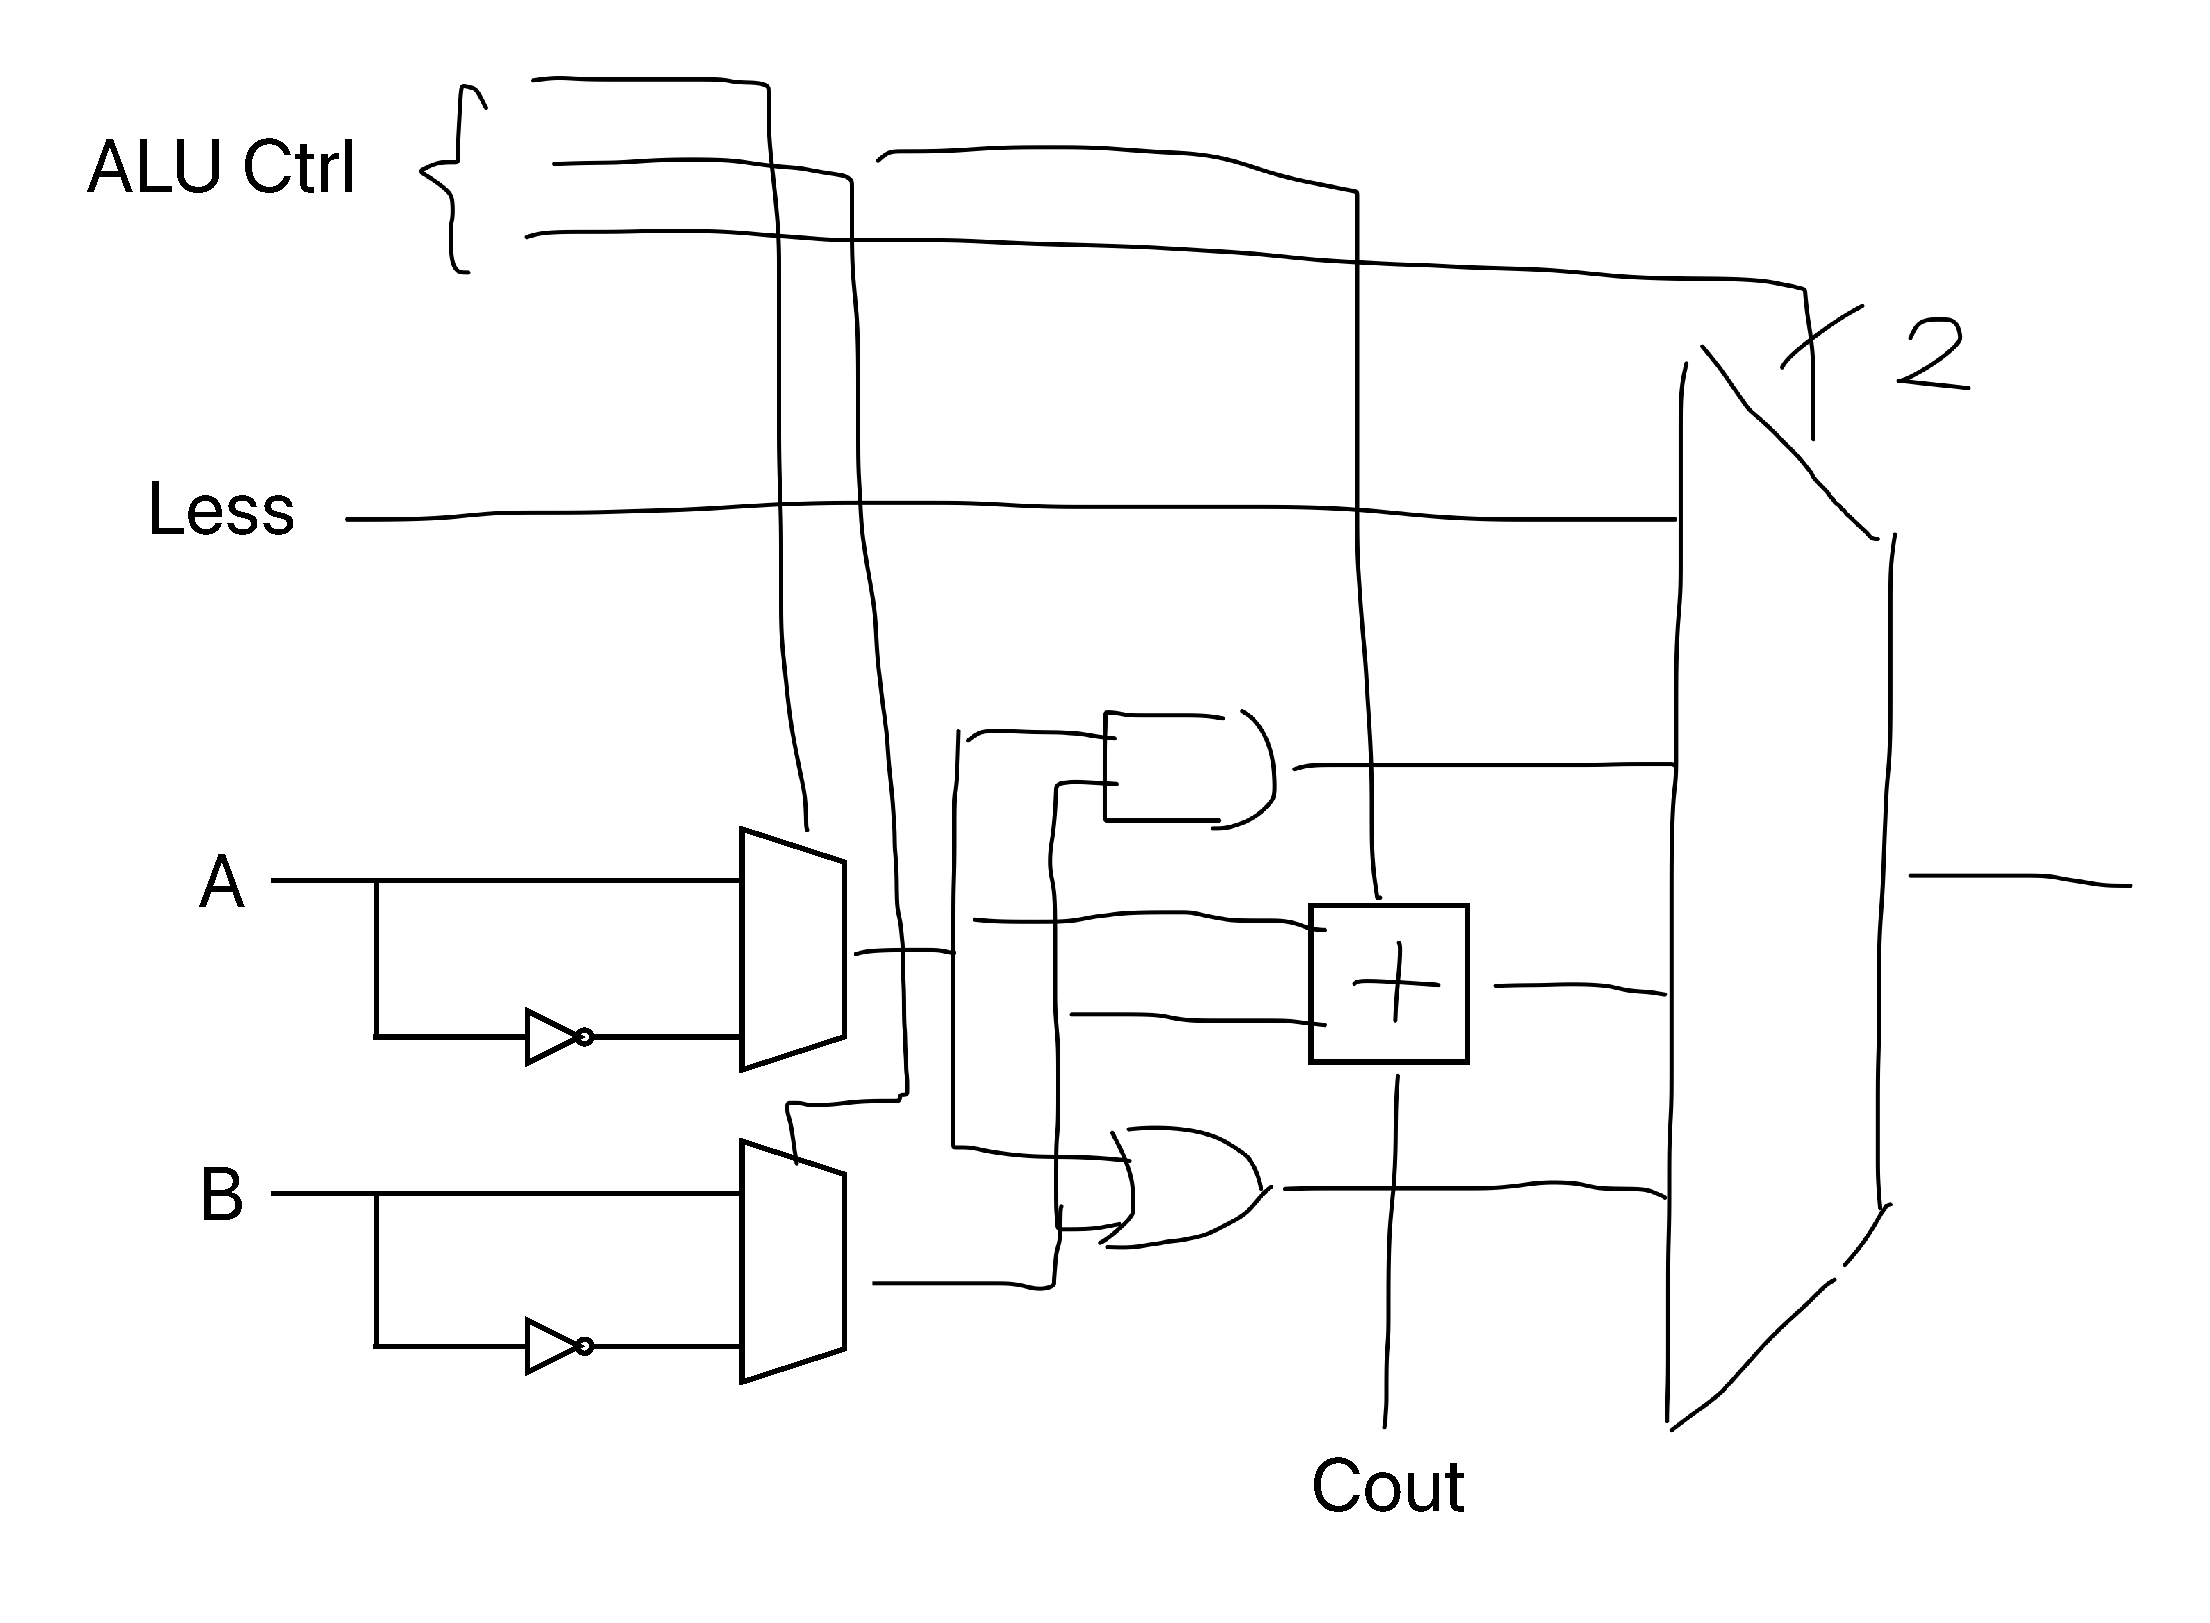
\includegraphics[width=\linewidth]{Unsigned ALU 0}
\caption{Leftmost one}
\end{subfigure}
\begin{subfigure}{.45\linewidth}
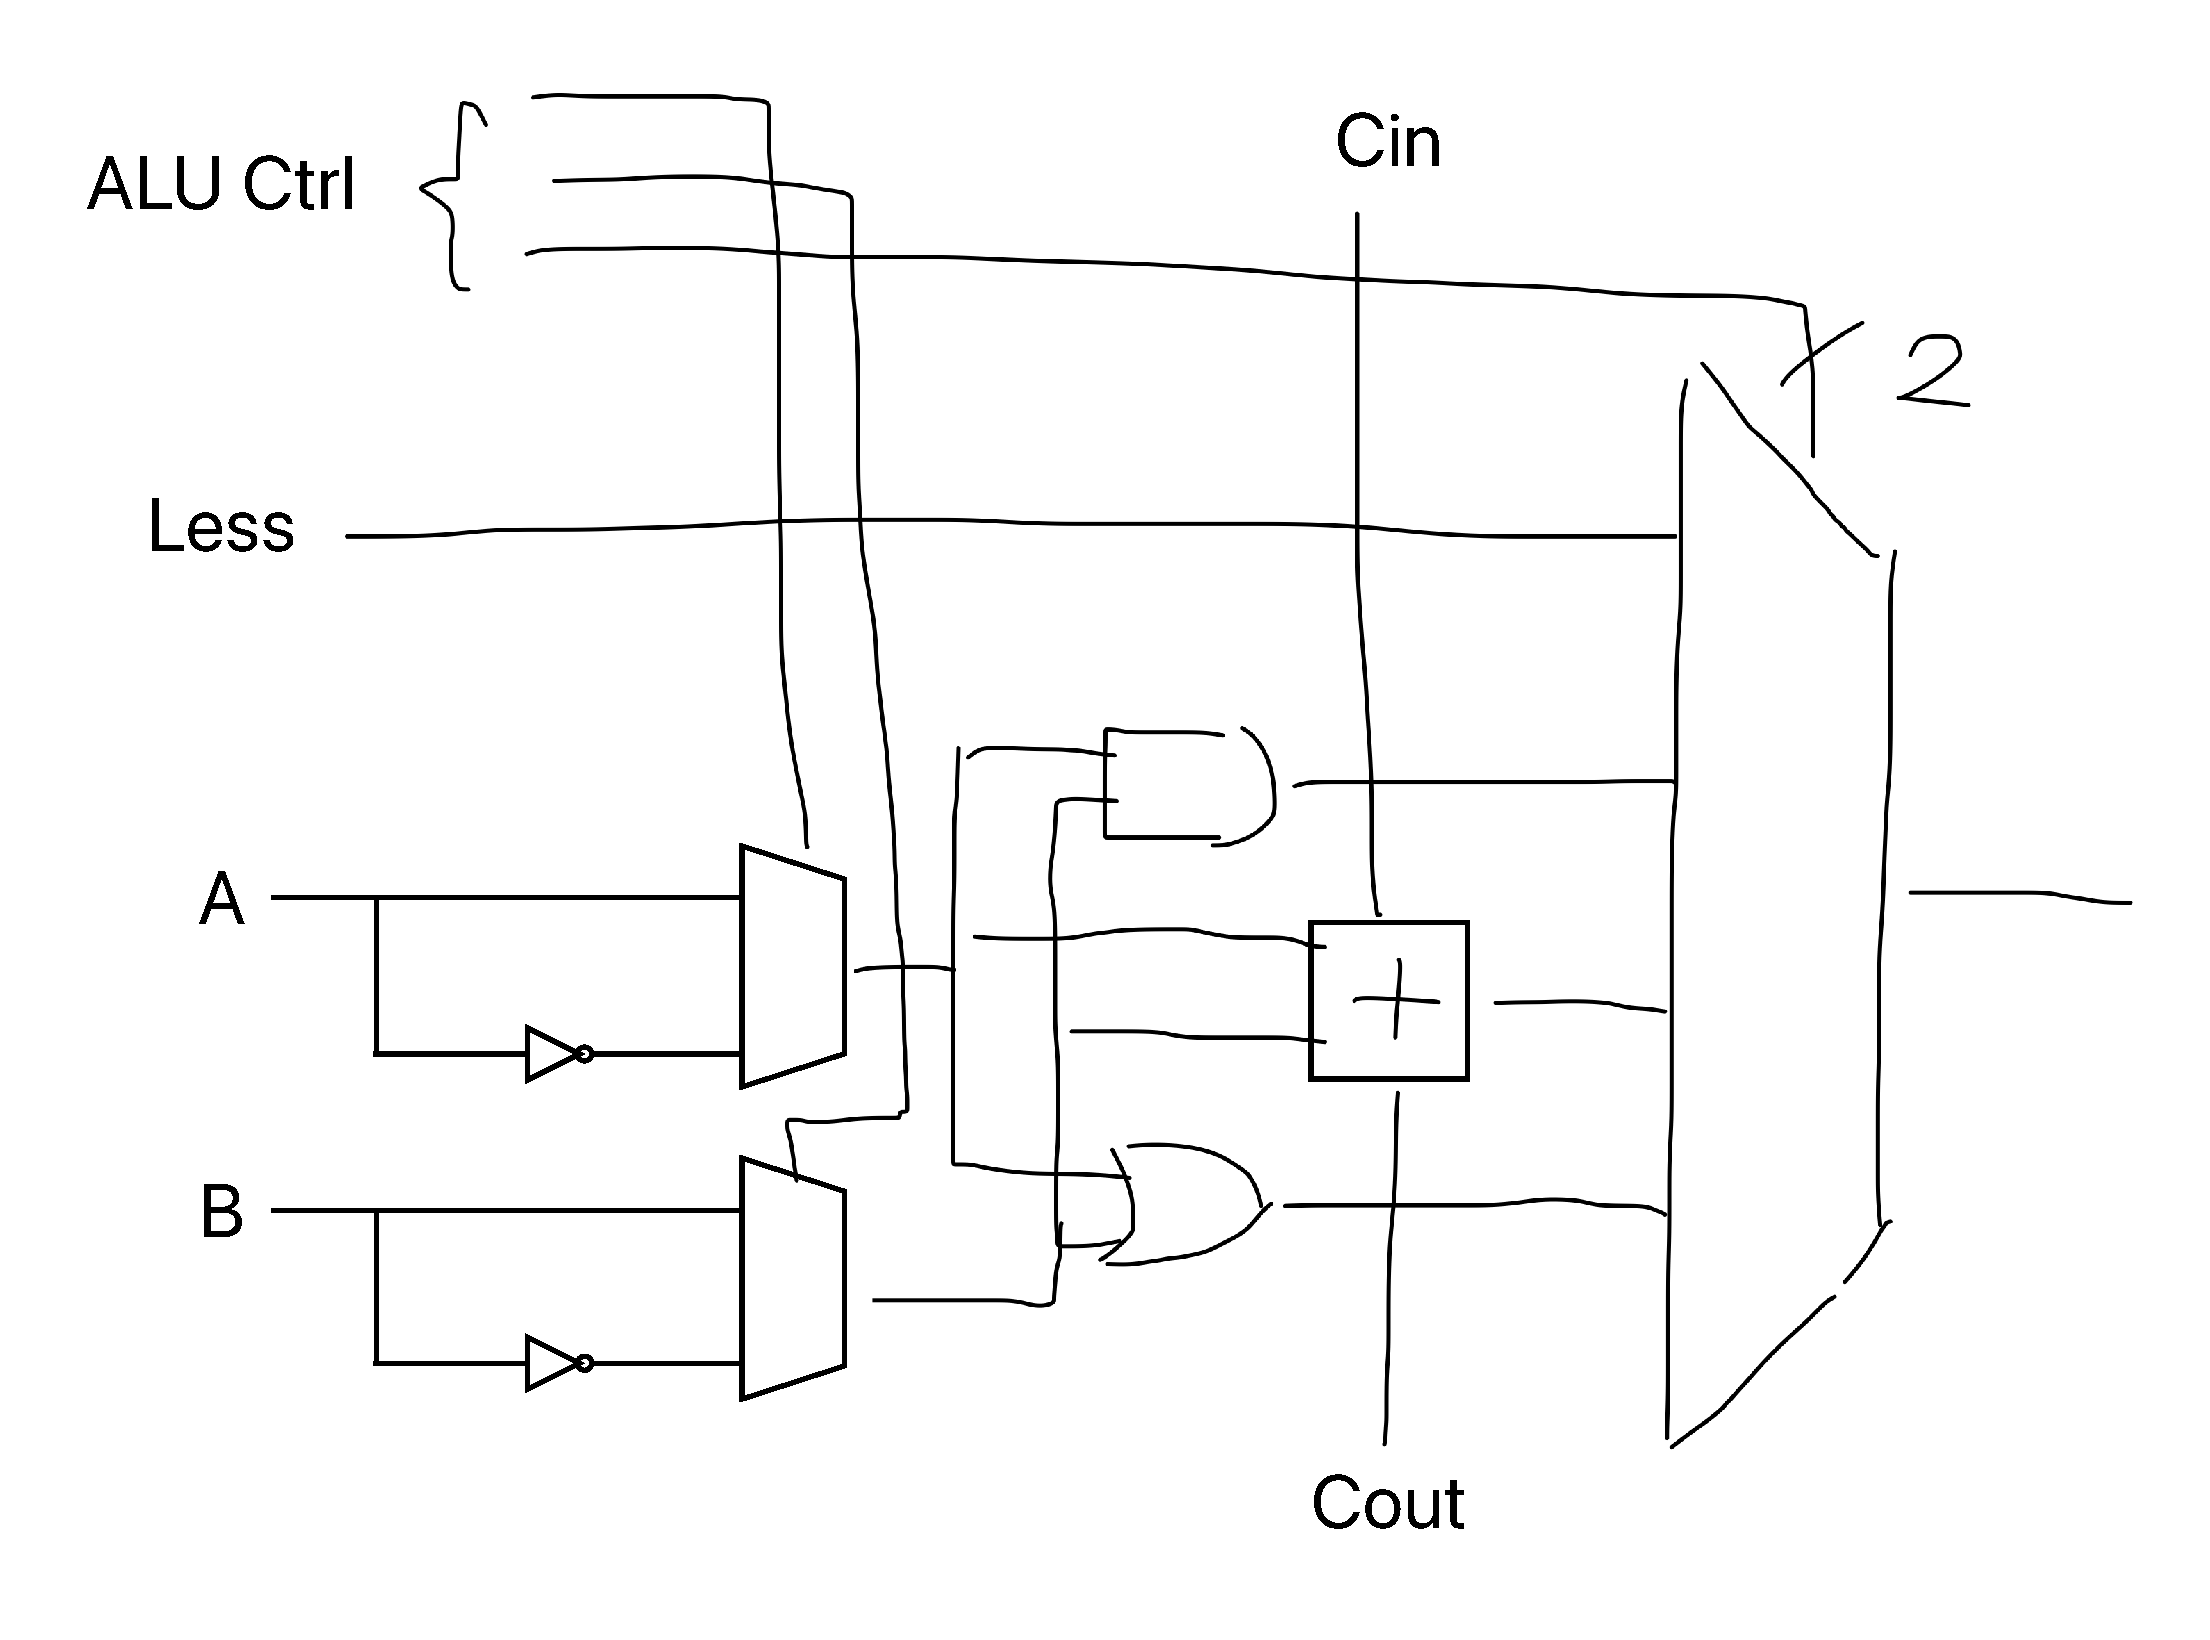
\includegraphics[width=\linewidth]{Unsigned ALU}
\caption{Others}
\end{subfigure}
\caption{1-bit unsigned ALU}
\label{fig:alu}
\end{figure}

\begin{figure}[H]
\centering
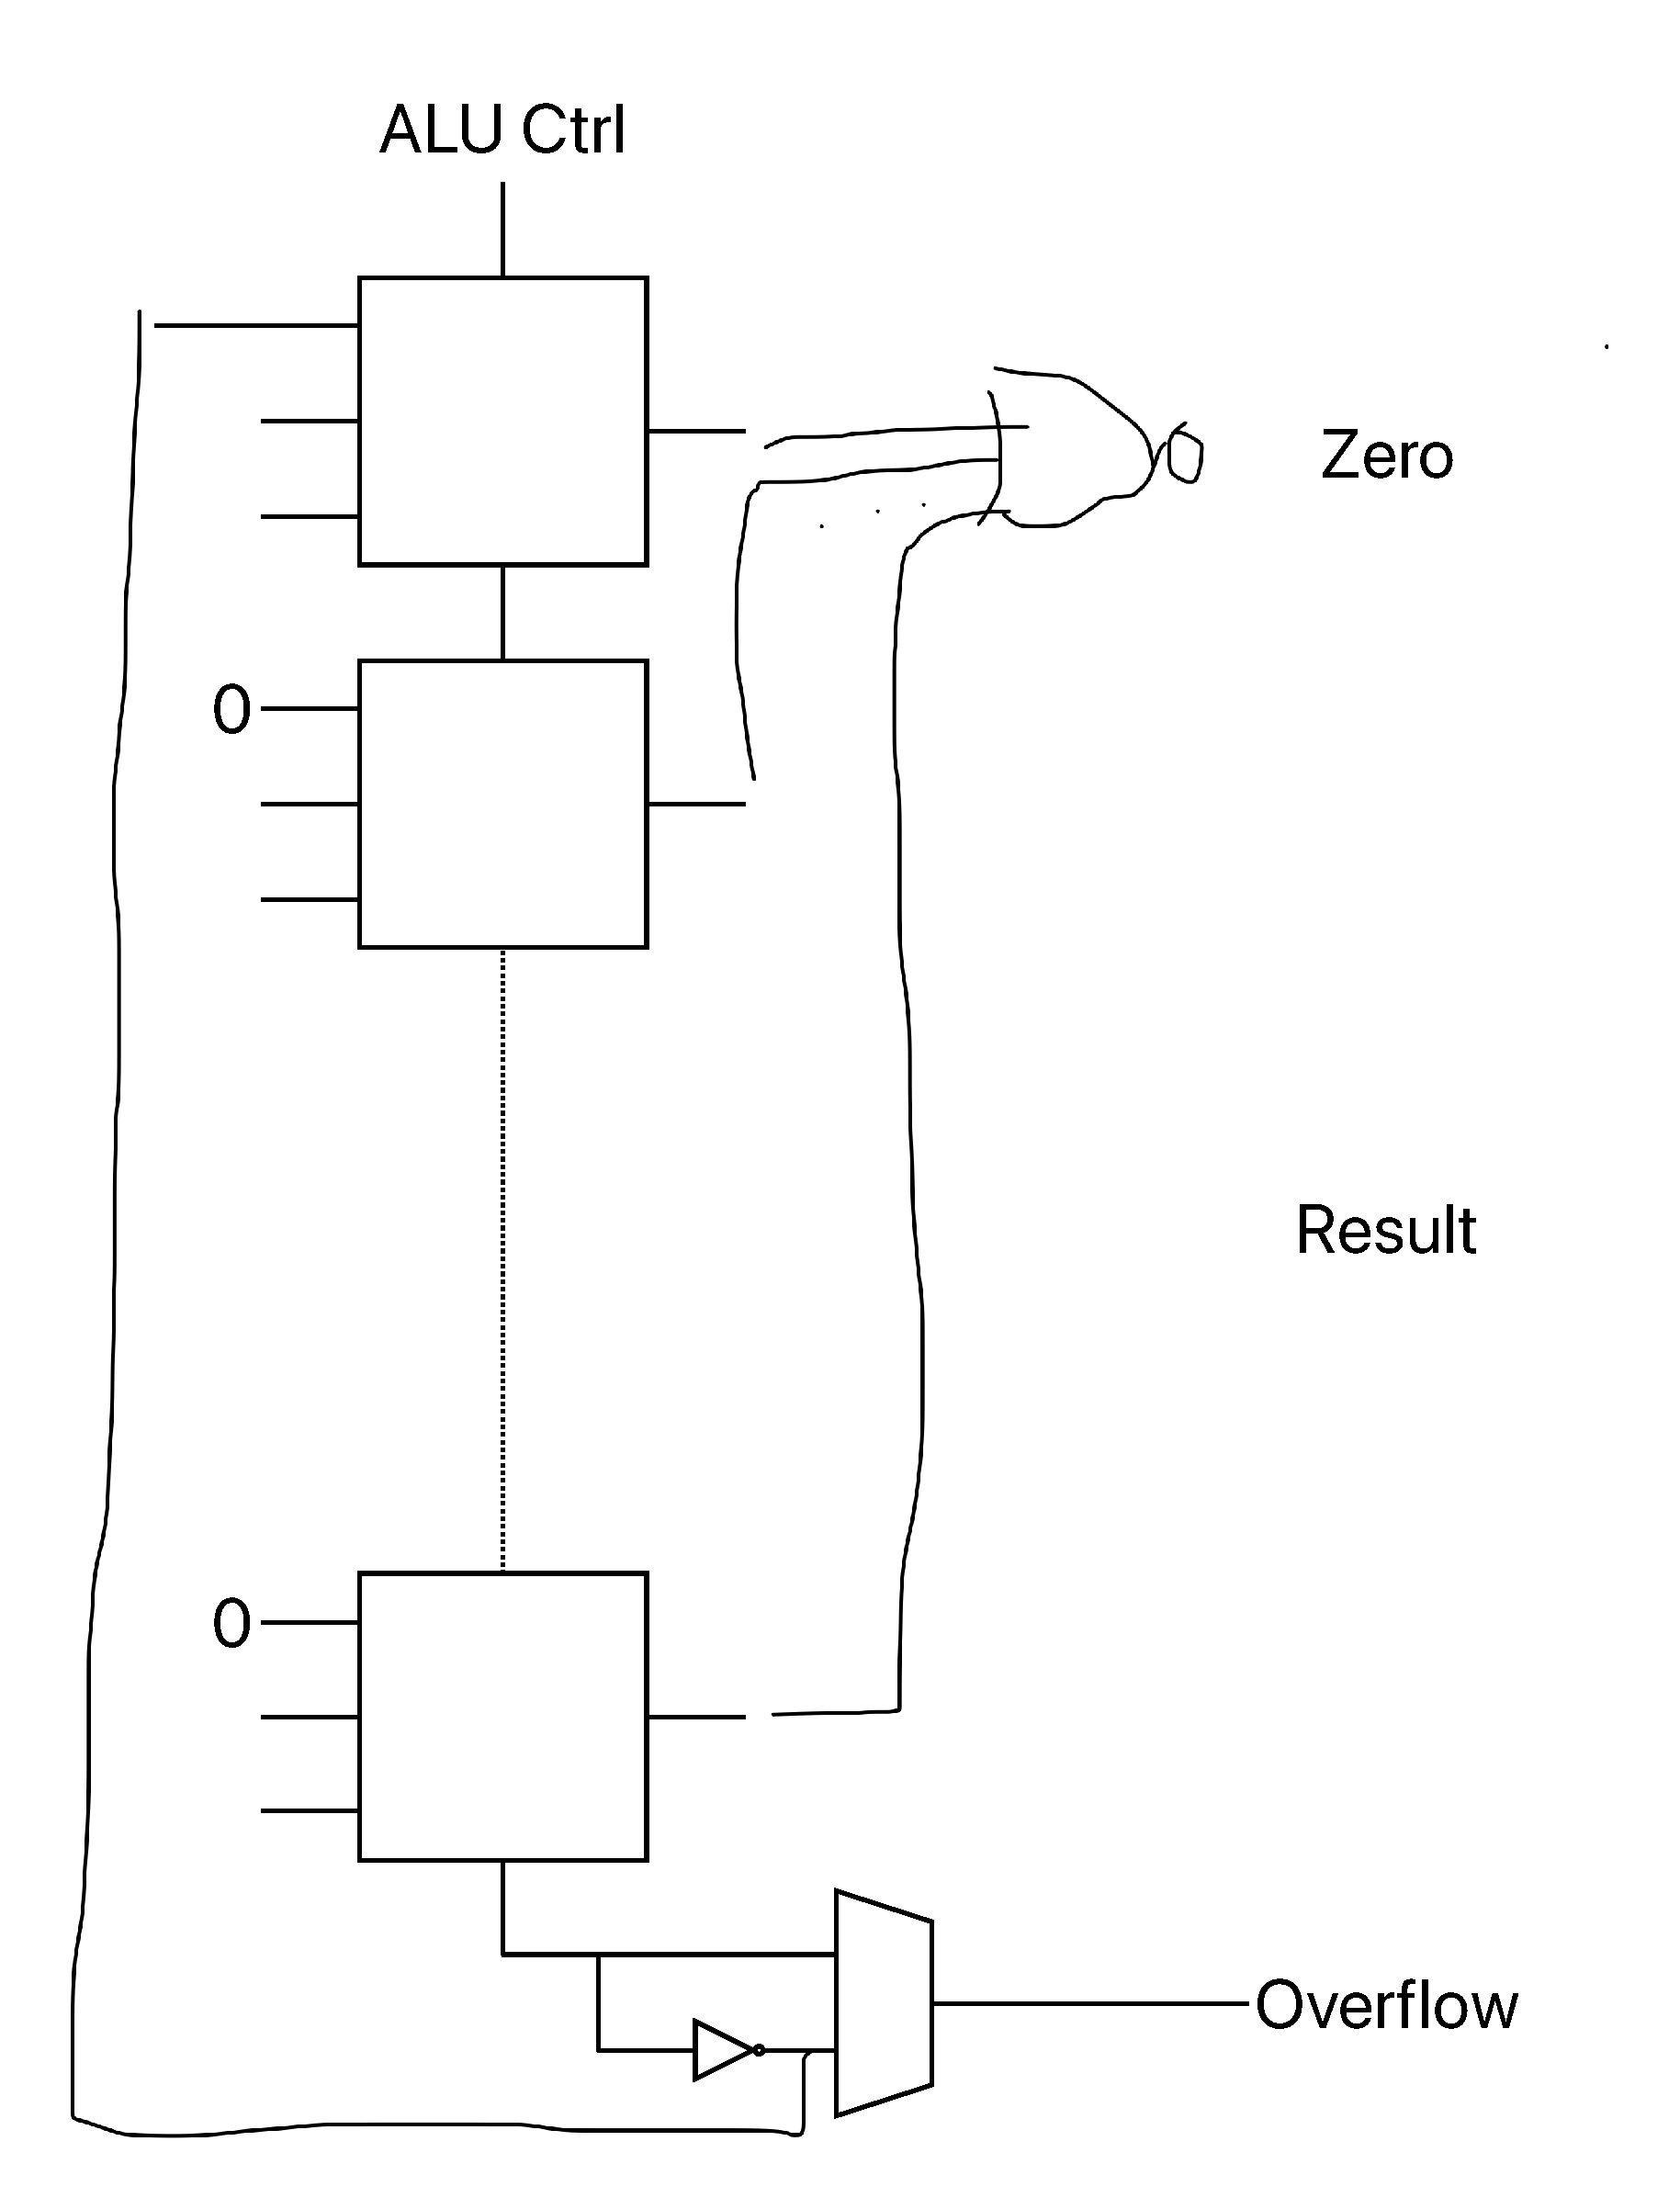
\includegraphics[width=\linewidth]{Unsigned ALU 64-bit}
\caption{64-bit unsigned ALU}
\label{fig:alu64}
\end{figure}

\section{Multiplications}

\subsection{Ver. 1}

\begin{table}[htp]
\caption{Multiplication Ver. 1}
\label{tab:multiply1}
\centering
\begin{tabular}{ccc}
\hline
Multiplicand & Multiplier & Product \\
\hline
0000 0111 & 1101 & 0000 0111 \\
0000 1110 & 0110 & 0000 0111 \\
0001 1100 & 0011 & 0010 0011 \\
0011 1000 & 0001 & 0101 1011 \\
0111 0000 & 0000 & 0101 1011 \\
\hline
\end{tabular}
\end{table}

\subsection{Ver. 2}

\begin{table}[htp]
\caption{Multiplication Ver. 2}
\label{tab:multiply2}
\centering
\begin{tabular}{cc}
\hline
Multiplicand & Product / Multiplier \\
\hline
0111 & 011\underline{1 110}1 \\
0111 & 001\underline{11 11}0 \\
0111 & 100\underline{011 1}1 \\
0111 & 101\underline{1011} 1 \\
0111 & 01011011 \\
\hline
\end{tabular}
\end{table}

The 4 underlined bits in each row are the rightmost 4 bits in the next row. By adding the left 3 bits of the product and the multiplicand, we could obtain the left half of the next product.

\section{Divisions}

\subsection{Ver. 1}

\begin{table}[H]
\caption{Division Ver. 1}
\label{tab:divide1}
\centering
\begin{tabular}{ccc}
\hline
Remainder & Divisor & Quotient \\
\hline
0000 0111 & 0110 0000 & 0000 \\
0000 0111 & 0011 0000 & 0000 \\
0000 0111 & 0001 1000 & 0000 \\
0000 0111 & 0000 1100 & 0000 \\
0000 0001 & 0000 0110 & 0001 \\
\hline
\end{tabular}
\end{table}

\subsection{Ver. 2}

\begin{table}[htp]
\caption{Division Ver. 2}
\label{tab:divide2}
\centering
\begin{tabular}{cc}
\hline
Remainder / Quotient & Divisor \\
\hline
\underline{0000}111 0 & 0110 \\
\underline{0001}11 00 & 0110 \\
\underline{0011}1 000 & 0110 \\
\underline{0111} 0000 & 0110 \\
0001 0001 & 0110 \\
\hline
\end{tabular}
\end{table}

Initially, the remainder is shifted left by 1 bit. In each row, we check whether the leftmost 4 bits of remainder are greater than or equal to the divisor. If true, the former would be subtracted by the latter and we append 1 to the quotient. Otherwise, we append 0 to the quotient.

\section{IEEE 754 Single Precision}

\subsection{Two Floating-point Numbers}

$$X=0.3125=\frac{3125}{10^4}=\frac{5^5}{2^4\times5^4}=\frac{5}{2^4}=5\times2^{-4}=(4+1)\times2^{-4}$$
$$Y=-15.98765=-\frac{1598765}{10^5}=-\frac{511\times5^5}{2^5\times5^5}=-(\sum_{i=0}^82^i)\times2^{-5}$$

And $-2+127=125_{10}=01111101_2$, $3+127=130_{10}=10000010_2$.

\begin{table}[htp]
\caption{Bit Representations}
\label{tab:represent}
\centering
\begin{tabular}{cccc}
\hline
 & Sign & Exponent & Fraction \\
\hline
$X$ & 0 & 01111101 & 01000000000000000000000 \\
$Y$ & 1 & 10000010 & 11111111000000000000000 \\
\hline
\end{tabular}
\end{table}

\subsection{Their Sum}

\begin{enumerate}
\item Align exponents. So $X$ equals \texttt{0 10000010 00001010000000000000000}.
\item Add fractions. We get \texttt{11110101000000000000000}.
\item Normalised result. Not necessary in this case.
\item Round. Not necessary, too.
\end{enumerate}

Hence we have $X+Y=$ \texttt{1 10000010 11110101000000000000000}.

\subsection{Their Product}

\begin{enumerate}
\item Add exponents. We get $-2+3=1$.
\item Multiply fractions. $1.01_2\times1.11111111_2=10.0111111011_2$.
\item Normalised result. The exponent increases by 1.
\item Round. Not necessary in this case.
\item Determine the sign. It's negative.
\end{enumerate}

Hence we have $X\times Y=$ \texttt{1 10000001 00111111011000000000000}.

\section{\textit{Quarter} Precision}

\subsection{Largest Negative ``Normalised'' Number $a_0$}

$$a_0=-1\times1\times2^{-2}$$

\subsection{Smallest Negative ``Denormalised'' Number $a_1$ \& 2\textsuperscript{nd} Smallest Negative ``Denormalised'' Number $a_2$}

$$a_1=-1\times(0.1111)_2\times2^{-2}$$
$$a_2=-1\times(0.1110)_2\times2^{-2}$$

\subsection{Difference Between $a_0$ \& $a_1$, $a_1$ \& $a_2$}

$$|a_2-a_1|=|a_1-a_0|=(0.0001)_2\times2^{-2}=2^{-6}$$

Denormalised numbers are distributed evenly between the largest negative normalised number and the smallest positive normalised number.

\subsection{Convert \texttt{0x5C}}

Since \texttt{0x5C = 0b 0 101 1100}, it represent $(1.1100)_2\times2^2=4+2+1=7$.

\subsection{Approximation $U$ for -5.7}

$$5.7=2^2+2^0+2^{-1}+2^{-3}+2^{-4}+\dots\approx(1.0110\ 110)_2\times2^2$$

Since guard bit, round bit are both 1, we take $U=(1.0111)_2\times2^2=5.75$. So the error is 0.05.

\section{Compare \texttt{float}s}

The function would return true if and only if any of the following conditions is satasified:
\begin{itemize}
\item Both $x,y$ are 0.
\item $x\geq0\land y\leq0$
\item $x\geq0\land y\geq0\land|x|\geq|y|$
\item $x\leq0\land y\leq0\land|x|\leq|y|$
\end{itemize}
These above cover all of the cases that $x\geq y$. Hence the claim is correct.

\end{document}
